\chapter{Thiết kế hệ thống phân loại tự động}
\paragraph{Giới thiệu} Vè nội dung chương này, chúng em sẽ miêu tả lại quá trình mà chúng em đã thiết kế nên hệ thống gồm các bước như cách áp dụng một số design pattern vào việc xây dựng hệ thống, các phác thảo sơ khai của giao diện, cách kết hợp các thư viện lập trình đã giới thiệu với Vaadin Framework và cuối cùng là thiết kế một ontology dùng để trình bày tính năng phân loại sau khi hệ thống được xây dựng thành công.
\section{Giải thích về việc lựa chọn nền tảng sử dụng}
Như đã được trình bày ở mục trên, Vaadin Framework là một nền tảng xây dựng Web dựa trên ngôn ngữ Java, nhưng không giống với phần lớn các framework Web khác vốn hoạt động theo mô hình Model-View-Controller (MVC). Vaadin chỉ cung cấp một bộ gồm rất nhiều UI Component có sẵn (đã được giải thích ở mục trước) làm cho việc xây dựng giao diện được đơn giản hóa một cách tối đa. Vì thế, lập trình viên sẽ không cần phải quan tâm nhiều đến HTML, JavaScript và ít phải quan tâm đến CSS, điều này giúp tập trung vào việc xây dựng logic của hệ thống tốt hơn. Việc thiết kế cho hệ thống này trên nền web sẽ tương tự như khi thiết kế một ứng dụng GUI trên nên Desktop nhờ có Vaadin.
\section{Thiết kế Use Case của hệ thống}
Trước tiên, chúng em giới thiệu một cách tổng quan về cách hệ thống hoạt động.
 \begin{figure}[ht!]
 	\centering
 	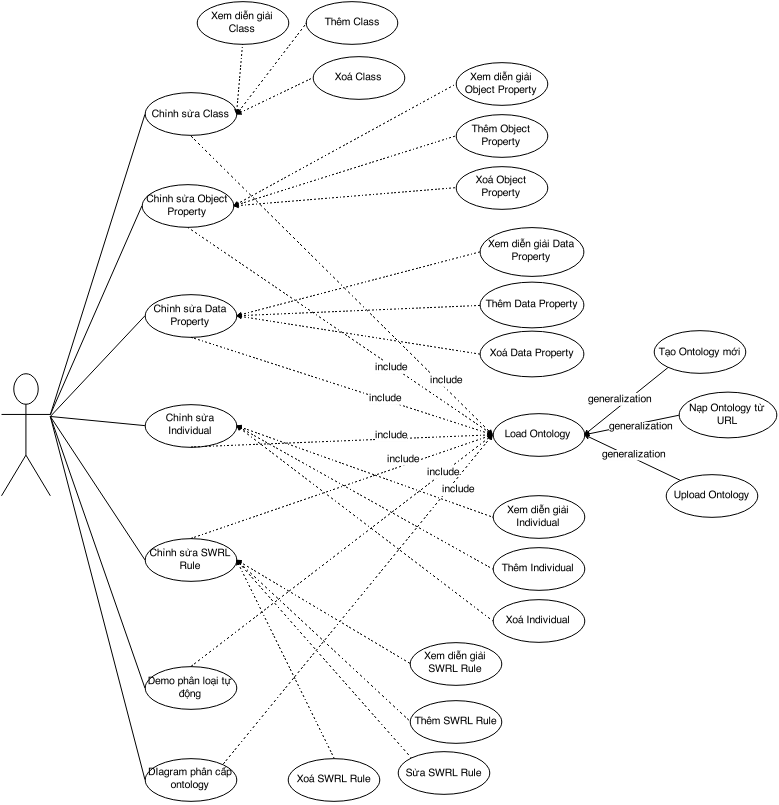
\includegraphics[width=155mm,height=170mm]{Figures/usecase.png}
 	\caption{Sơ đồ Use Case của hệ thống \label{overflow}}
 \end{figure}
\section{Thiết kế giao diện phác thảo}
Hệ thống hay ứng dụng sẽ gồm 2 view chính: view đầu tiên tạm gọi là EntryView dùng để nạp/tạo mới các tài liệu OWL 2. View thứ hai chính là view chính của ứng dụng gọi làm MainView cho phép thực hiện việc chỉnh sửa ontology, thực hiện suy luận (phục vụ cho tính năng phân loại). 
\begin{figure}[ht!]
	\centering
	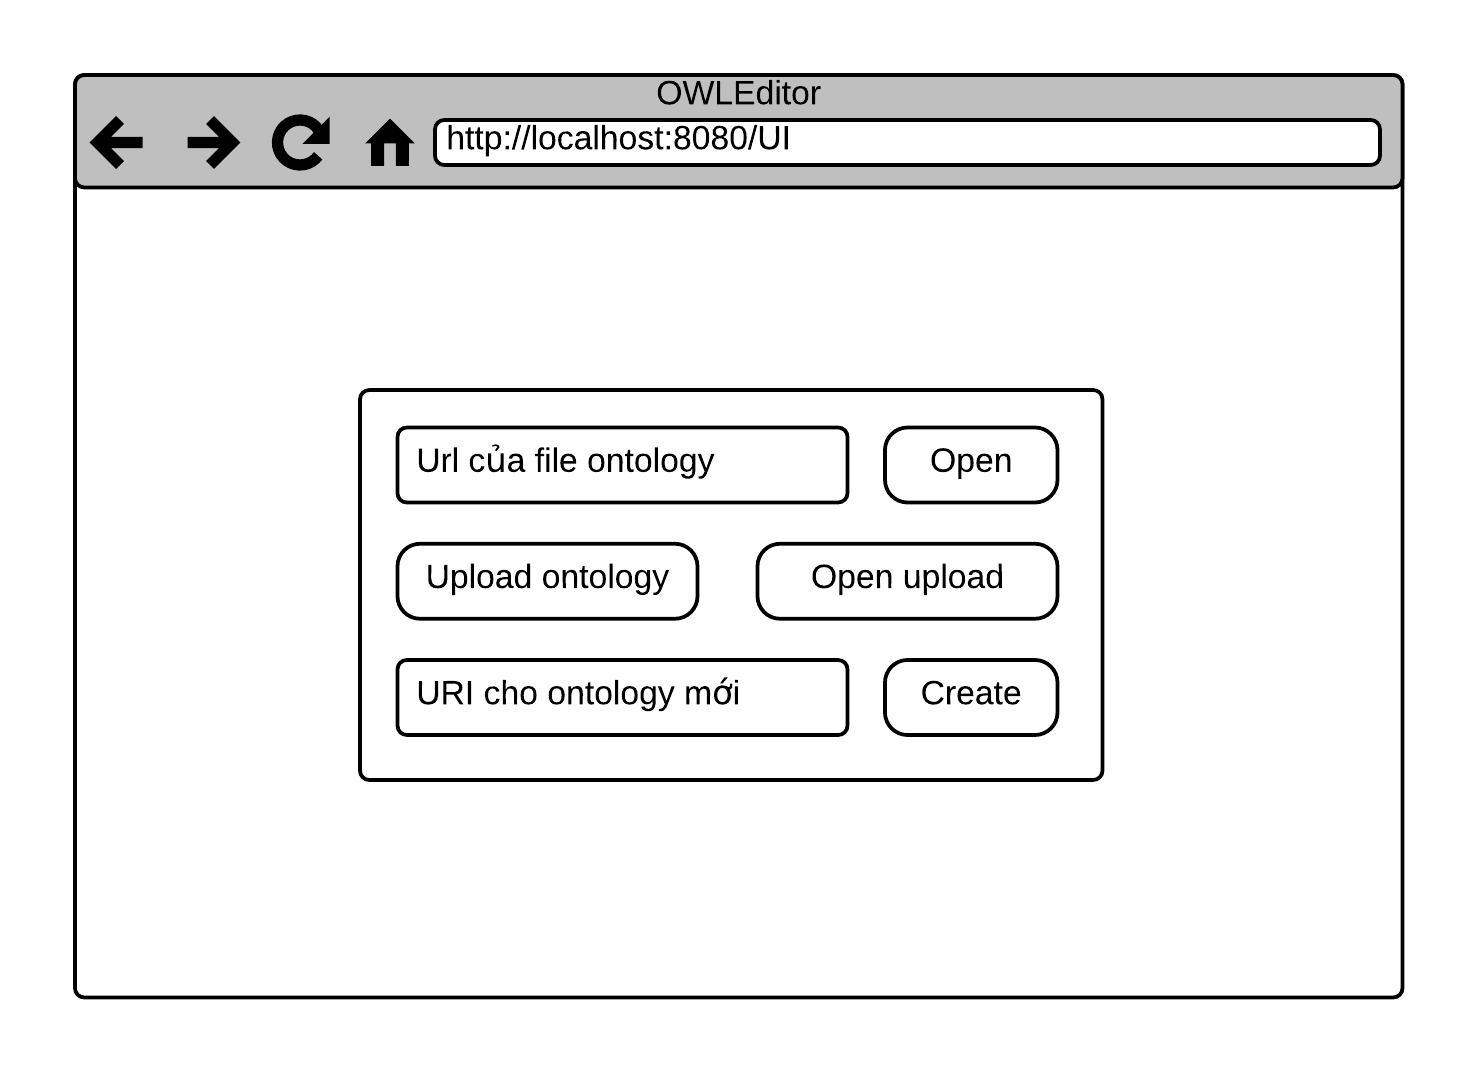
\includegraphics[width=150mm,height=95mm]{Figures/ui_entryview.png}
	\caption{Phác thảo Entry View \label{overflow}}
\end{figure}
MainView sẽ gồm nhiều tab, mỗi loại thực thể (gồm lớp, thuộc tính đối tượng, thuộc tính dữ liệu, cá thể) và SWRL Rule sẽ được tổ chức thành từng tab với tên tương ứng. 
\begin{figure}[h!]
	\centering
	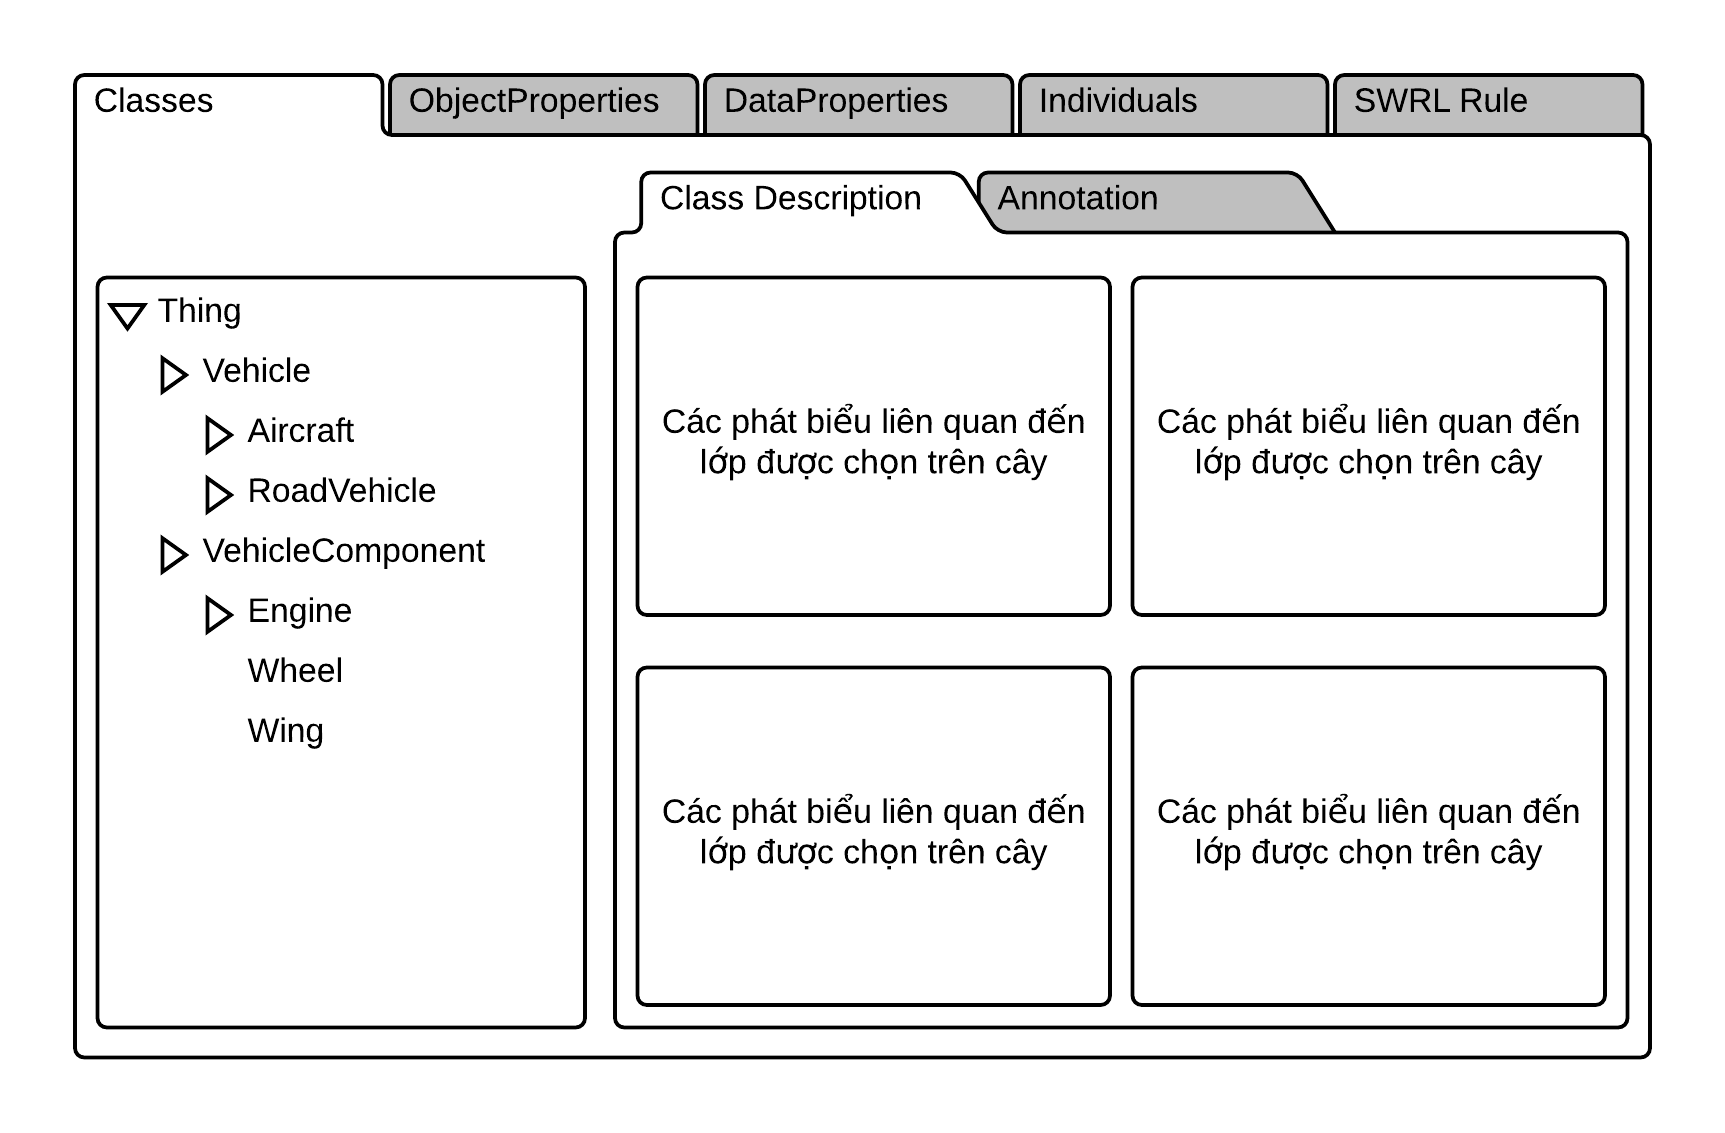
\includegraphics[width=150mm,height=95mm]{Figures/ui_mainview.png}
	\caption{Phác thảo Main View - Tab "Classes" (chứa lớp và các mô tả lớp liên quan) \label{overflow}}
\end{figure}
\begin{figure}[h!]
	\centering
	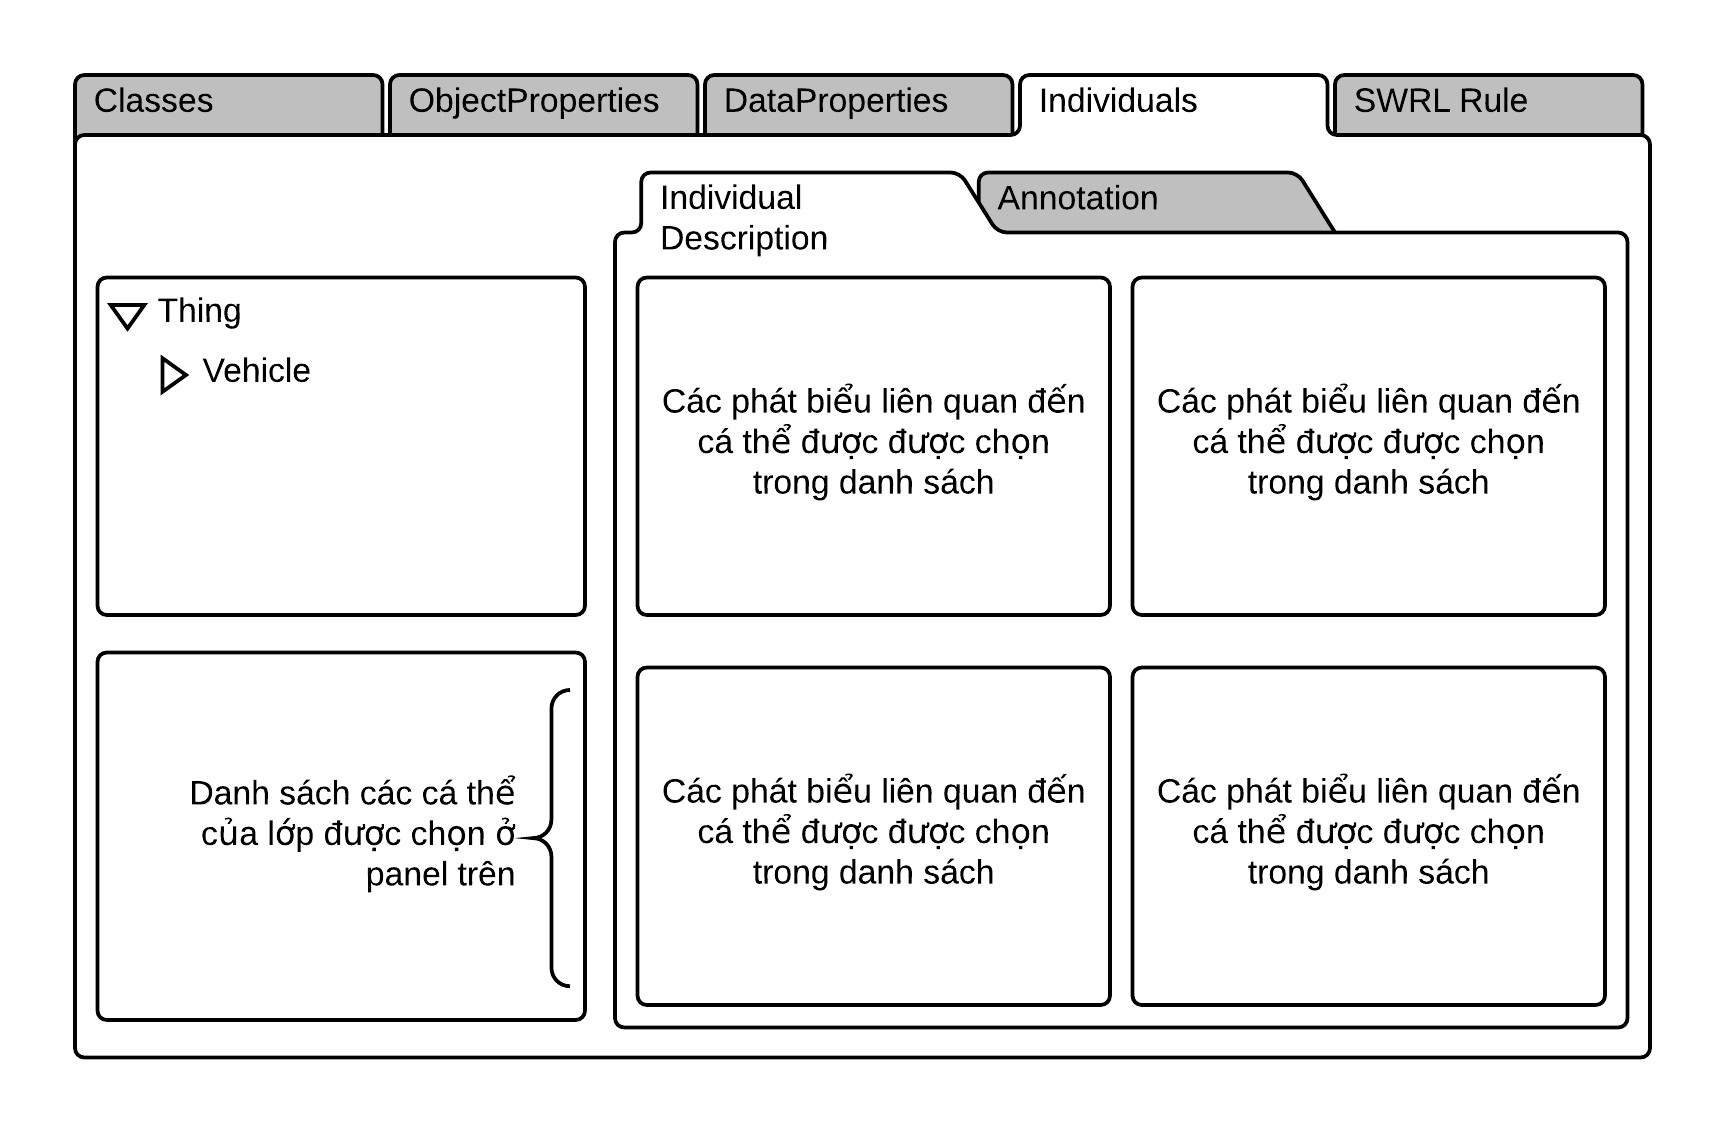
\includegraphics[width=150mm,height=95mm]{Figures/ui_mainview_individual.png}
	\caption{Phác thảo Main View - Tab "Individuals" (chứa cá thể và các mô tả liên quan) \label{overflow}}
\end{figure}
\begin{figure}[h!]
	\centering
	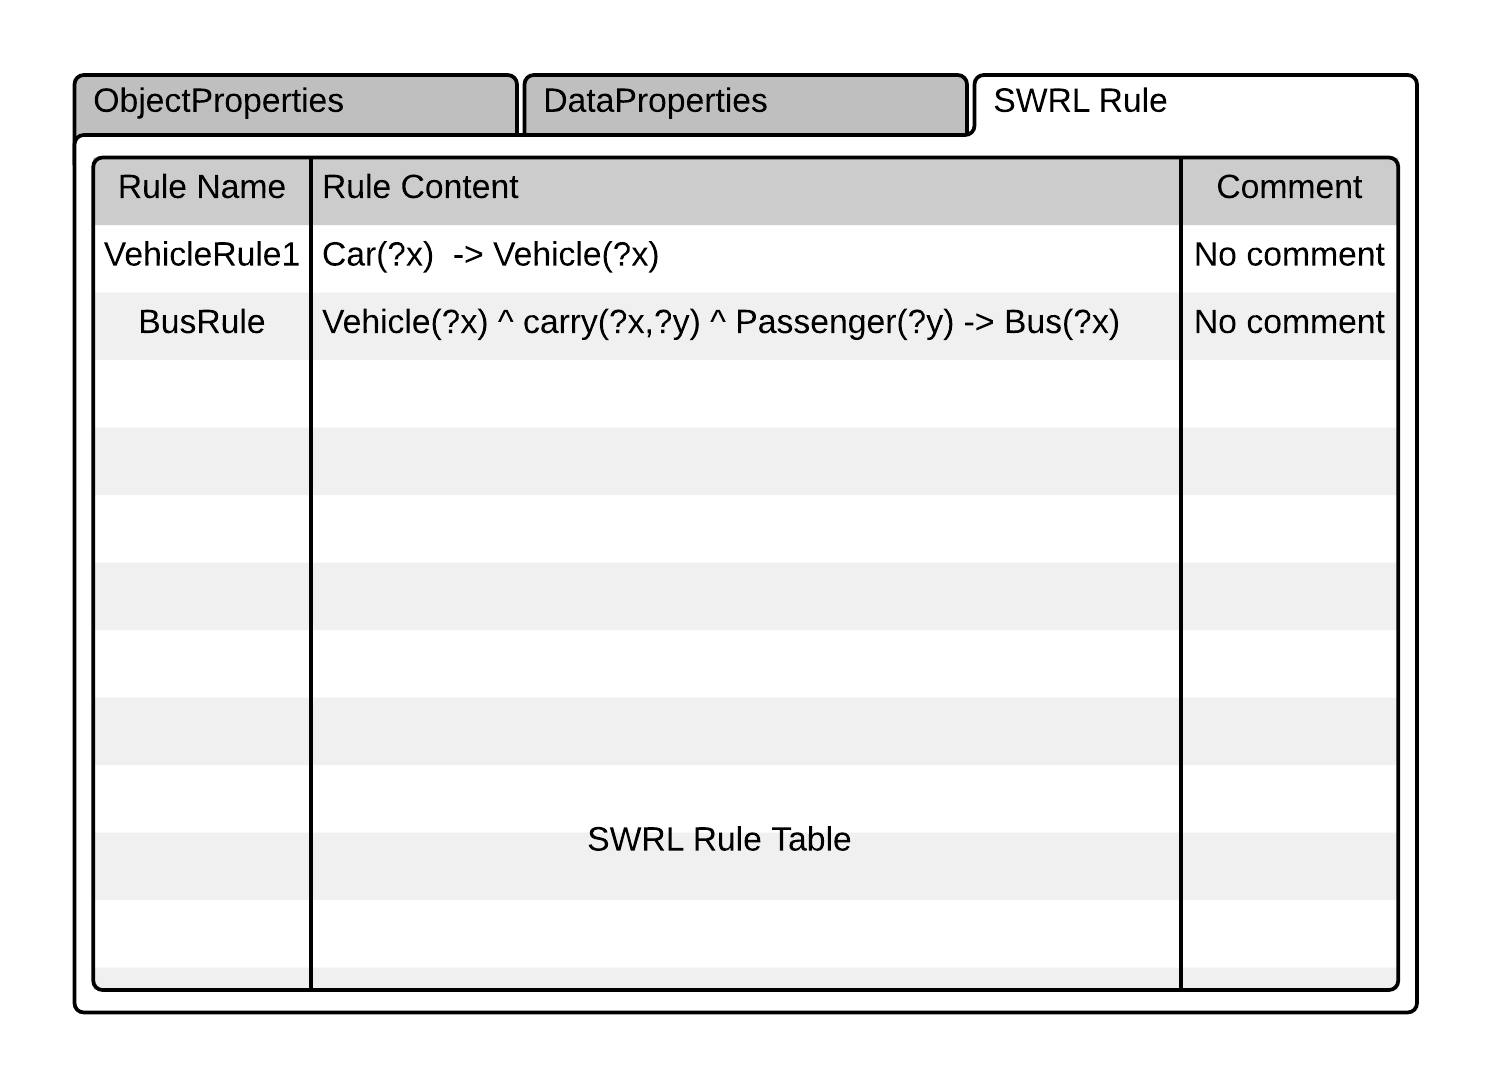
\includegraphics[width=150mm,height=95mm]{Figures/ui_mainview_swrltab.png}
	\caption{Phác thảo Main View - Tab "SWRL Rules" \label{overflow}}
\end{figure}
Các tab về lớp (Class), thuộc tính đối tượng (Object Propery) và thuộc tính dữ liệu (Data Propery) sẽ có bố cục giống nhau (Hình 3.3). Bên trái là một cây biểu diễn cấu trúc phân cấp của các loại thực thể này và bên phải là các panel nhỏ. Từng panel sẽ tương ứng với từng loại phát biểu có liên quan đến thực thể được chọn bên trái. Riêng tab về các cá thể sẽ có bố cục hơi khác so với các thực thể còn lại, nó sẽ có thêm một danh sách (sẽ nằm bên dưới cấu trúc cây chứa các lớp - Hình 3.4). Bên trong tab SWRL Rules sẽ là một bảng gồm chứa các rule, chia thành 3 cột gồm tên, nội dung và lời chú thích cho rule (Hình 3.5).
\begin{figure}[h!]
	\centering
	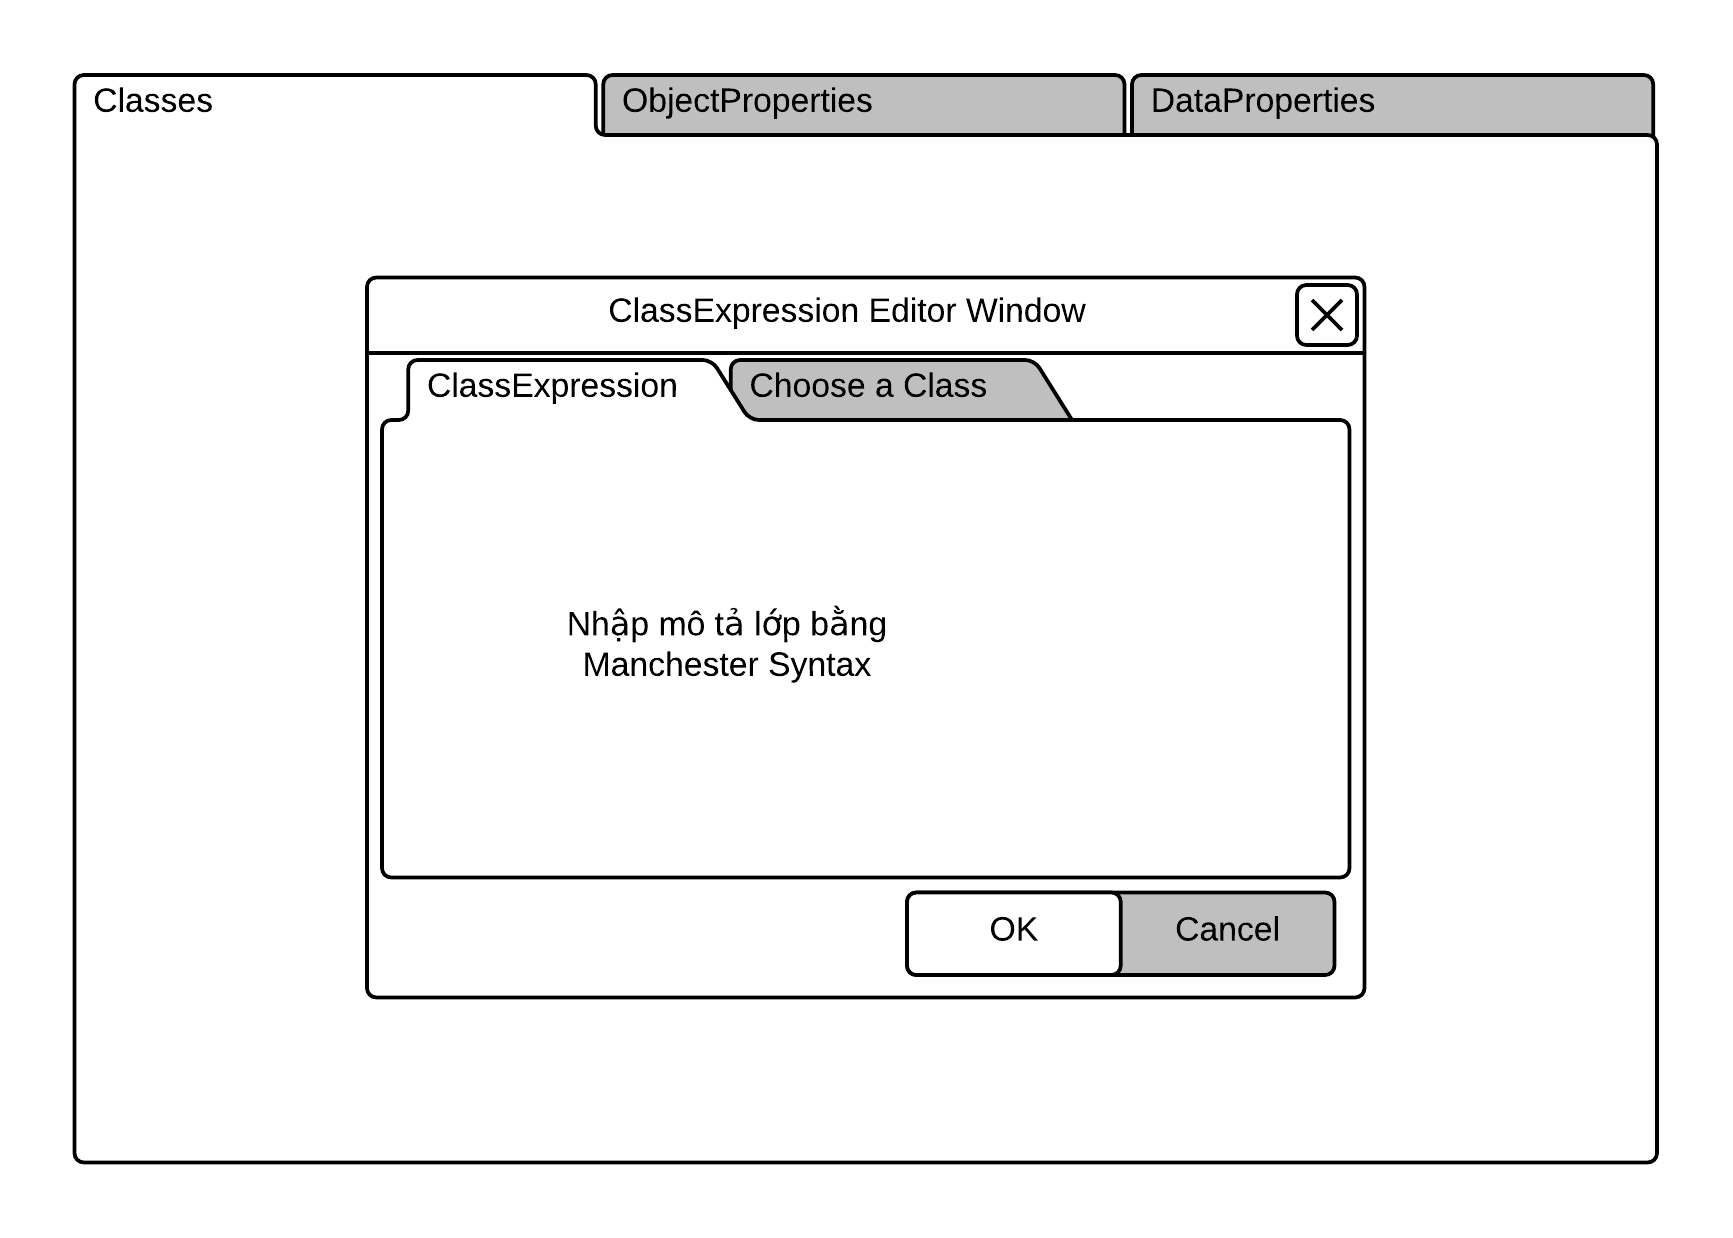
\includegraphics[width=150mm,height=100mm]{Figures/ui_classexpressioneditor.png}
	\caption{Phác thảo cửa sổ biên tập mô tả lớp\label{overflow}}
\end{figure}
\begin{figure}[h!]
	\centering
	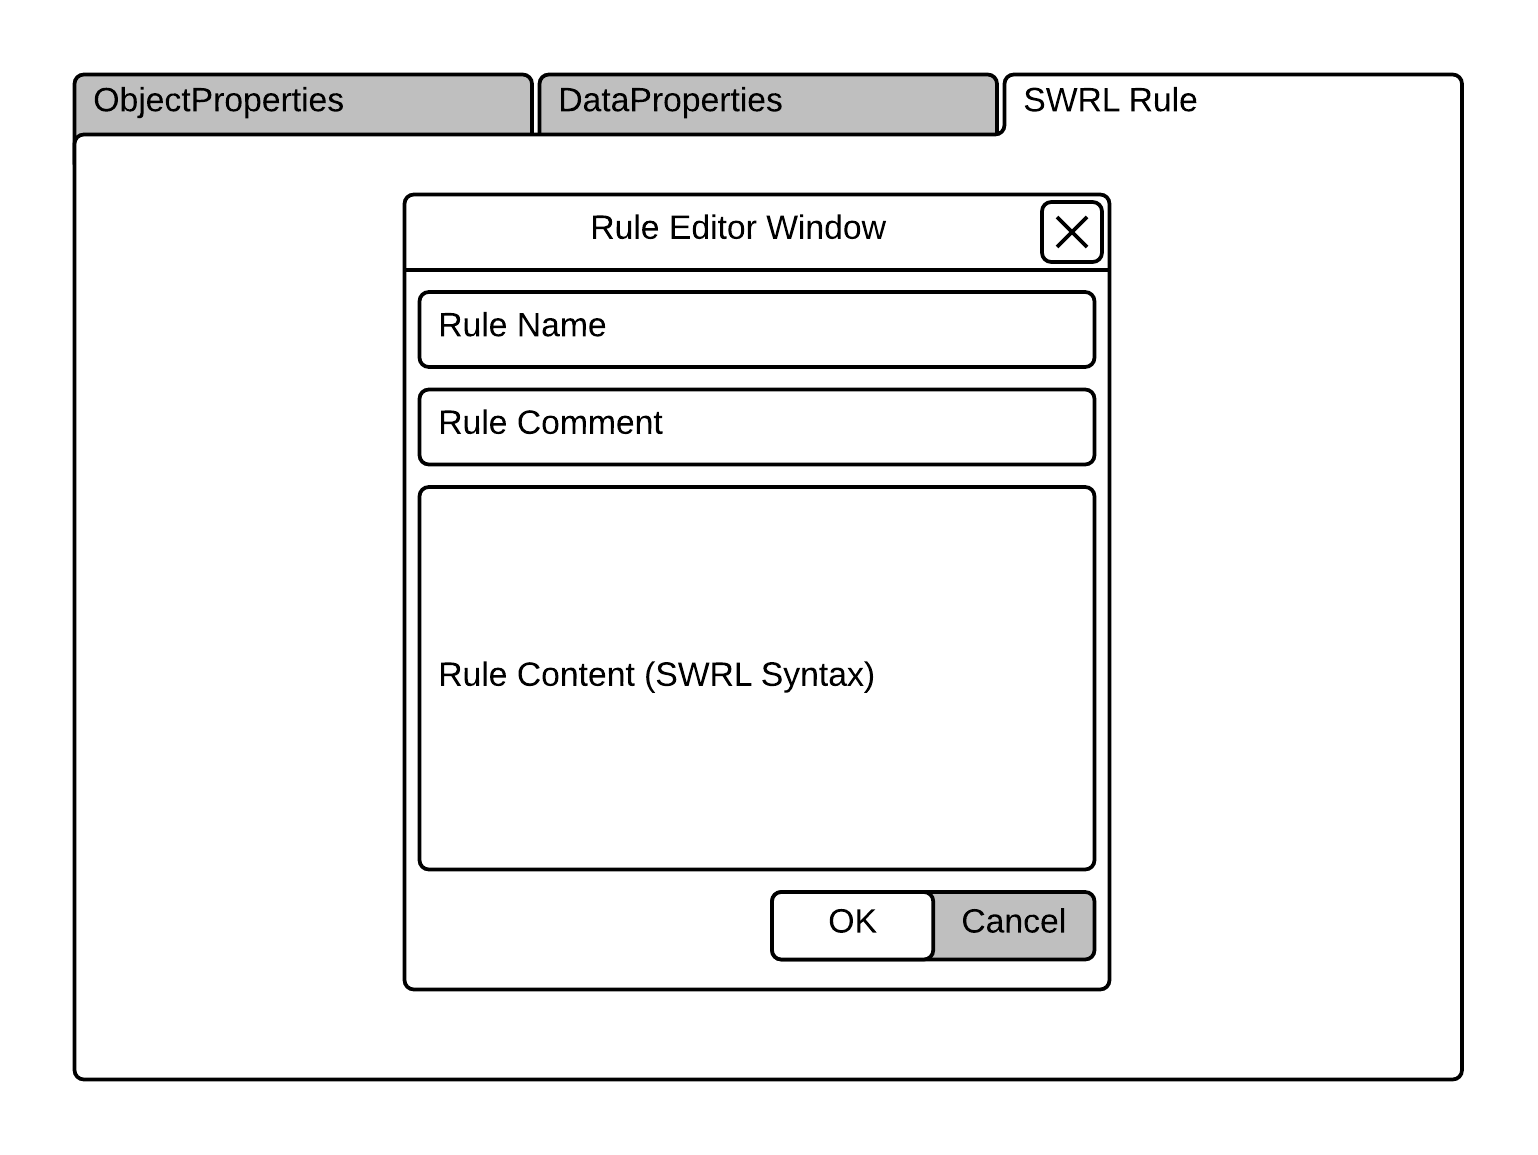
\includegraphics[width=155mm,height=95mm]{Figures/ui_mainview_ruleeditor.png}
	\caption{Phác thảo cửa sổ biên tập rule \label{overflow}}
\end{figure}
Ngoài các view và tab đã kể ở trên, thì ứng dụng buộc phải có thêm các thành phần giao diện hỗ trợ viêc biên tập mô tả lớp, thuộc tính, cá thể (class/property expression, individual assertion axiom) và việc biên tập SWRL Rule. Các hình 3.6, 3.7  thể hiện phác thảo về các giao diện đảm nhiệm những tính năng vừa nêu.
\section{Truy xuất đến các thành phần của Ontology trong OWL-API bằng cách áp dụng Visitor Pattern}
Trong OWL-API, các đối tượng dữ liệu có cấu trúc tương tự với các thành phần trong OWL 2 Ontology (được trình bày trong mục 2.2.3) - tên của các đối tượng dữ liệu sẽ có thêm tiếp đầu ngữ \textit{"OWL"} cộng với tên của thành phần trong OWL 2 như \textit{Ontology} thì đối tượng trong OWL-API sẽ là \textit{OWLOntology}, \textit{ClassExpression} (mô tả lớp) thì đối tượng tương ứng là \textit{OWLClassExpression}, tương tự cho các thành phần khác. Việc tương tác và thay đổi sẽ diễn ra trong đối tượng \textit{OWLOntology} - đối tượng Java biểu diễn một OWL 2 ontology. 
\\
Như đã được giới thiệu trong mục 2.2.3, với một cấu trúc phức tạp gồm nhiều đối tượng được mở rộng và thừa kế từ các loại đối tượng khác, thì việc truy xuất đến từng thành phần cụ thể và áp dụng các thay đổi khác nhau lên chúng là một tác vụ khó nếu không áp dụng Visitor Pattern.
\subsection{Visitor Pattern}
\begin{figure}[h!]
	\centering
	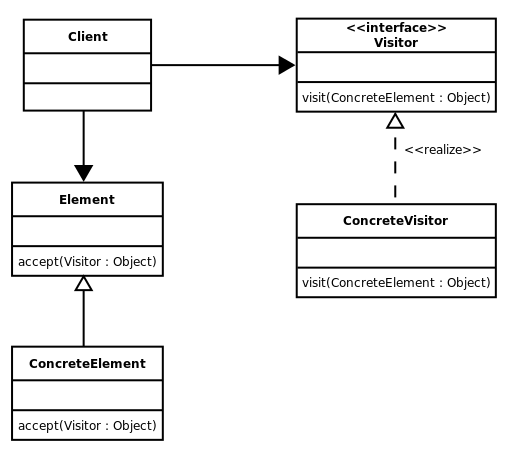
\includegraphics[width=100mm]{Figures/visitor_diagram.png}
	\caption{Visitor Design Pattern\label{overflow}}
\end{figure}
Visitor Pattern là một design pattern trong lập trình hướng đối tượng với mục tiêu tách biệt các cấu trúc dữ liệu khỏi giải thuật. Nói cách khác chúng ta dễ dàng thay đổi các giải thuật mong muốn lên các thành phần của OWLOntology mà không cần phải thay đổi cấu trúc của chúng. Như biểu diễn trong hình mọi loại đối tượng kế thừa/mở rộng từ IElement đều có khả năng truy xuất bởi các đối tượng áp dụng Interface Visitor, các giải thuật mong muốn sẽ được định nghĩa trong phương thức \textit{visit}.
\subsection{Visitor trong OWL-API}
Trong OWL-API cung cấp sẵn một số các Interface Visitor cho từng loại thành phần cụ thể. Ví dụ như OWLClassExpression sẽ có OWLClassExpressionVisitor, hay OWLDatatype sẽ có OWLDatatypeVisitor, .v.v.. . Hình sau đây miêu tả cách hoạt động của OWLClassExpressionVistor.
\begin{figure}[h!]
	\centering
	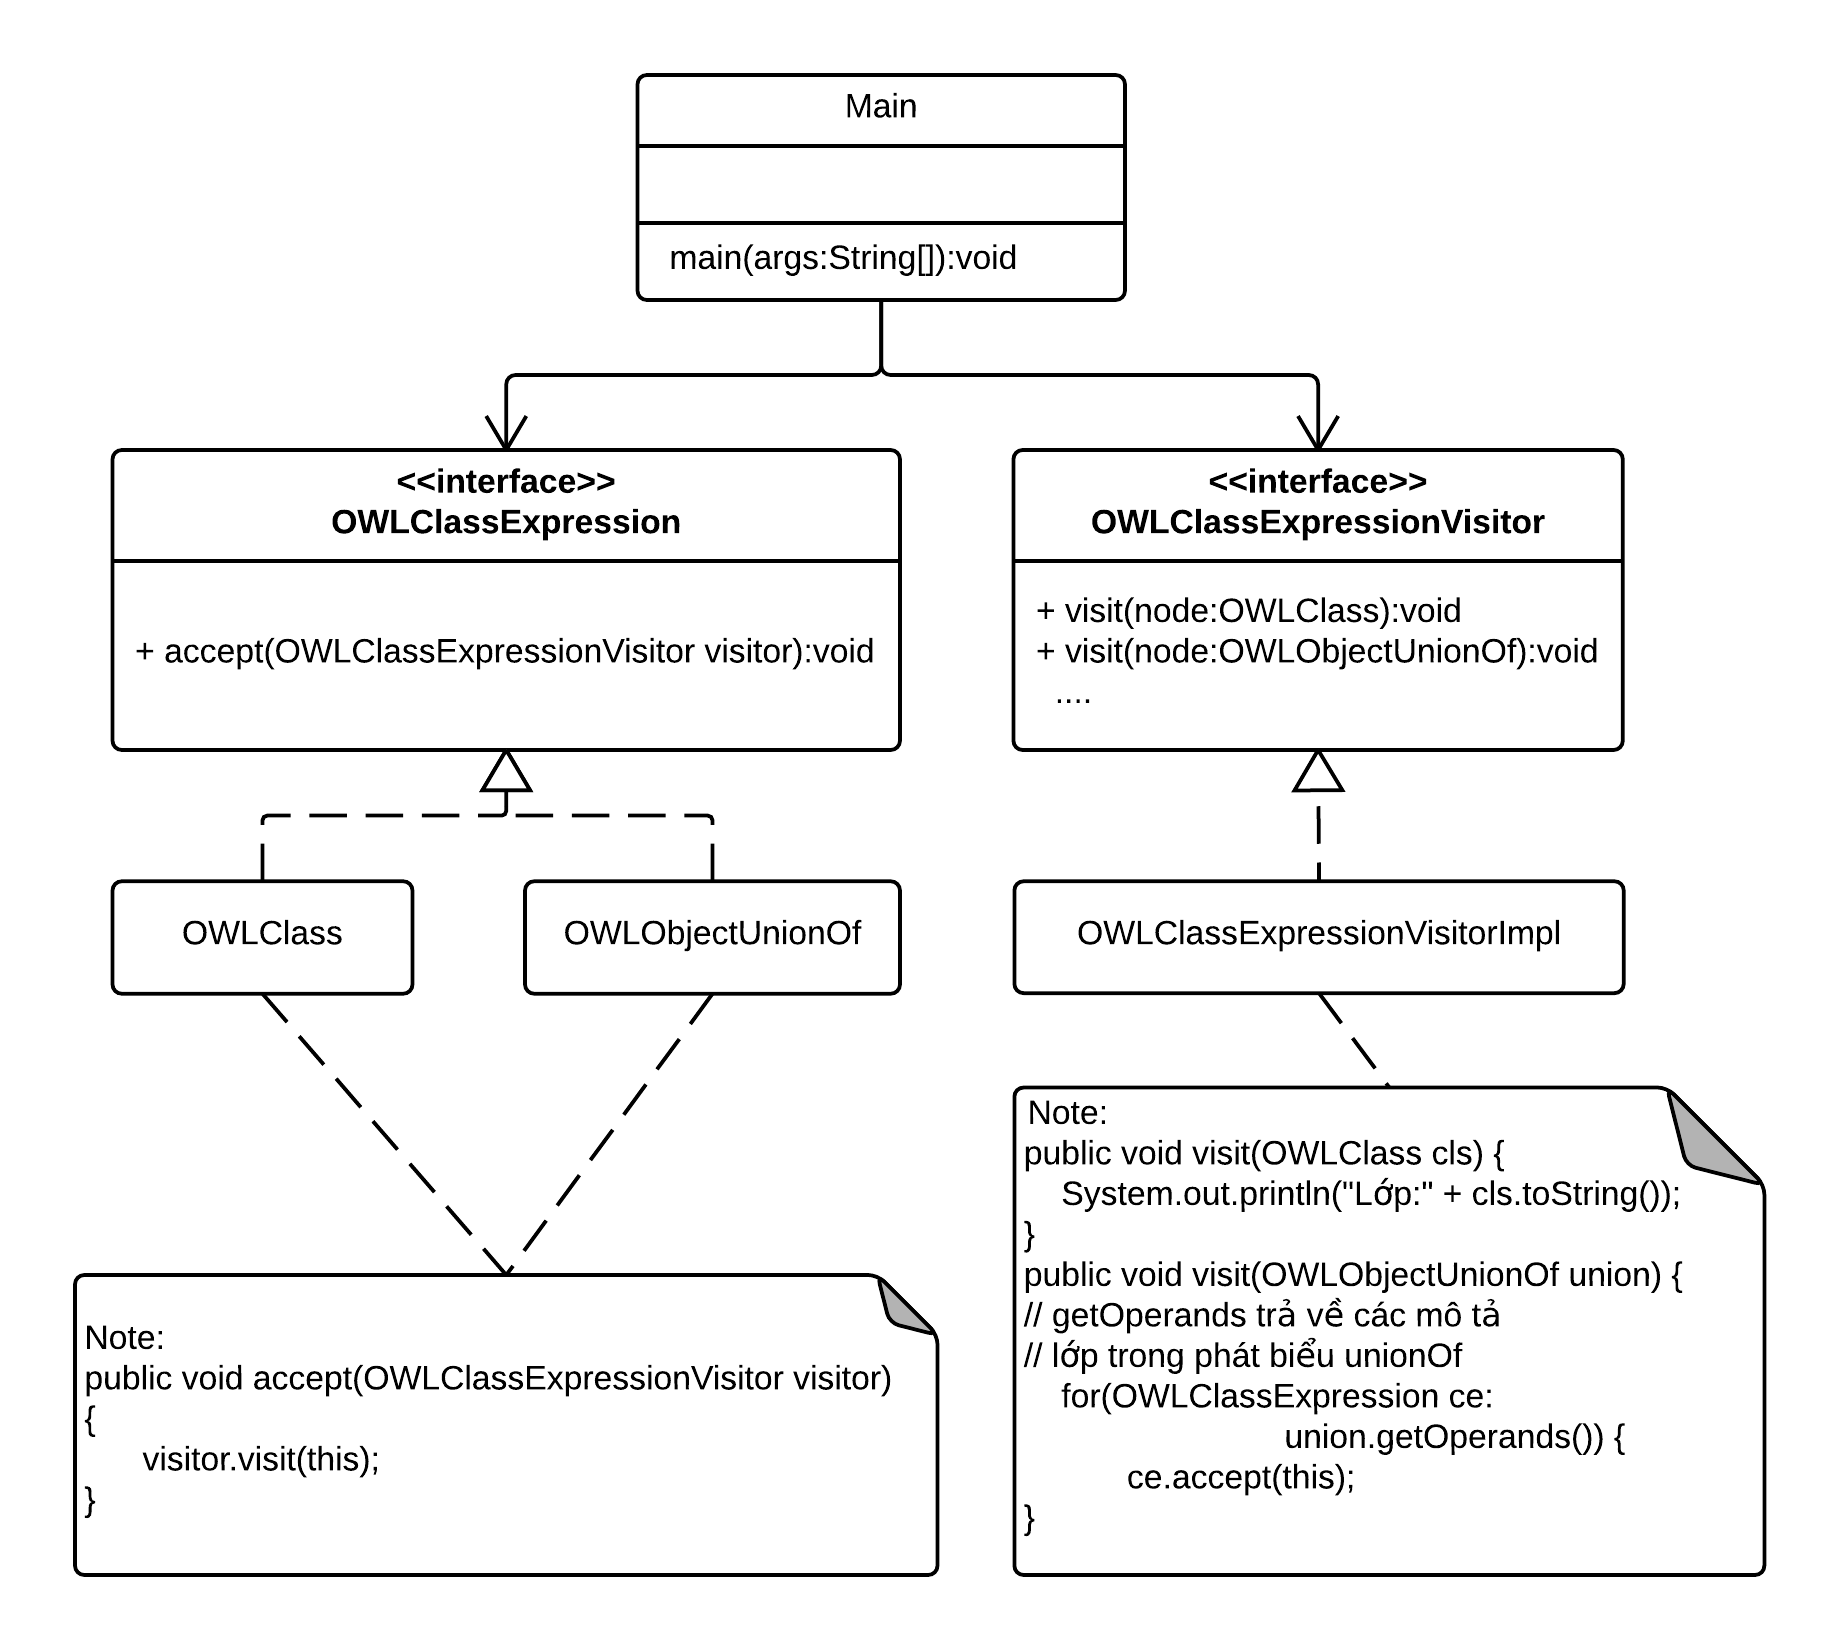
\includegraphics[width=145mm]{Figures/uml_classdiagram_classexpressionvistior_nobackground.png}
	\caption{OWLClassExpressionVisitor trong OWL-API \label{overflow}}
\end{figure}
{\let\thefootnote\relax\footnotetext{*\textit{
		OWLDataFactory: nằm trong OWL-API với chức năng dùng như một nhà máy tạo ra mọi loại đối tượng từ lớp, thuộc tính tới các phát biểu.
}}
Giải sử chúng ta có một mô tả lớp (class expression) bằng Manchester Syntax \textit{"Car and Bike"} và hàm main trong hình khai báo như sau:
\begin{verbatim}
// void main 
OWLDataFactory factory = OWLManager.getOWLDataFactory();
OWLClass car = factory.getOWLClass("a:Car");
OWLClass bike = factory.getOWLClass("a:Bike");
OWLObjectUnionOf union = factory.getOWLObjectUnionOf(car, bike);
OWLClassExpressionVisitor visitor = new OWLClassExpressionVisitorImpl();
union.accept(visitor);
// Ta sẽ có output là 
Lớp: a:Car
Lớp: a:Bike                                       
\end{verbatim}
Visitor lớn nhất trong OWL-API là \textit{OWLObjectVisitor} có khả năng truy vấn đến tất cả các loại đối tượng thuộc \textit{OWLOntology}. Visitor này thực ra được tập hợp lại từ nhiều visitor nhỏ hơn (Hình 3.10).
\begin{figure}[h!]
	\centering
	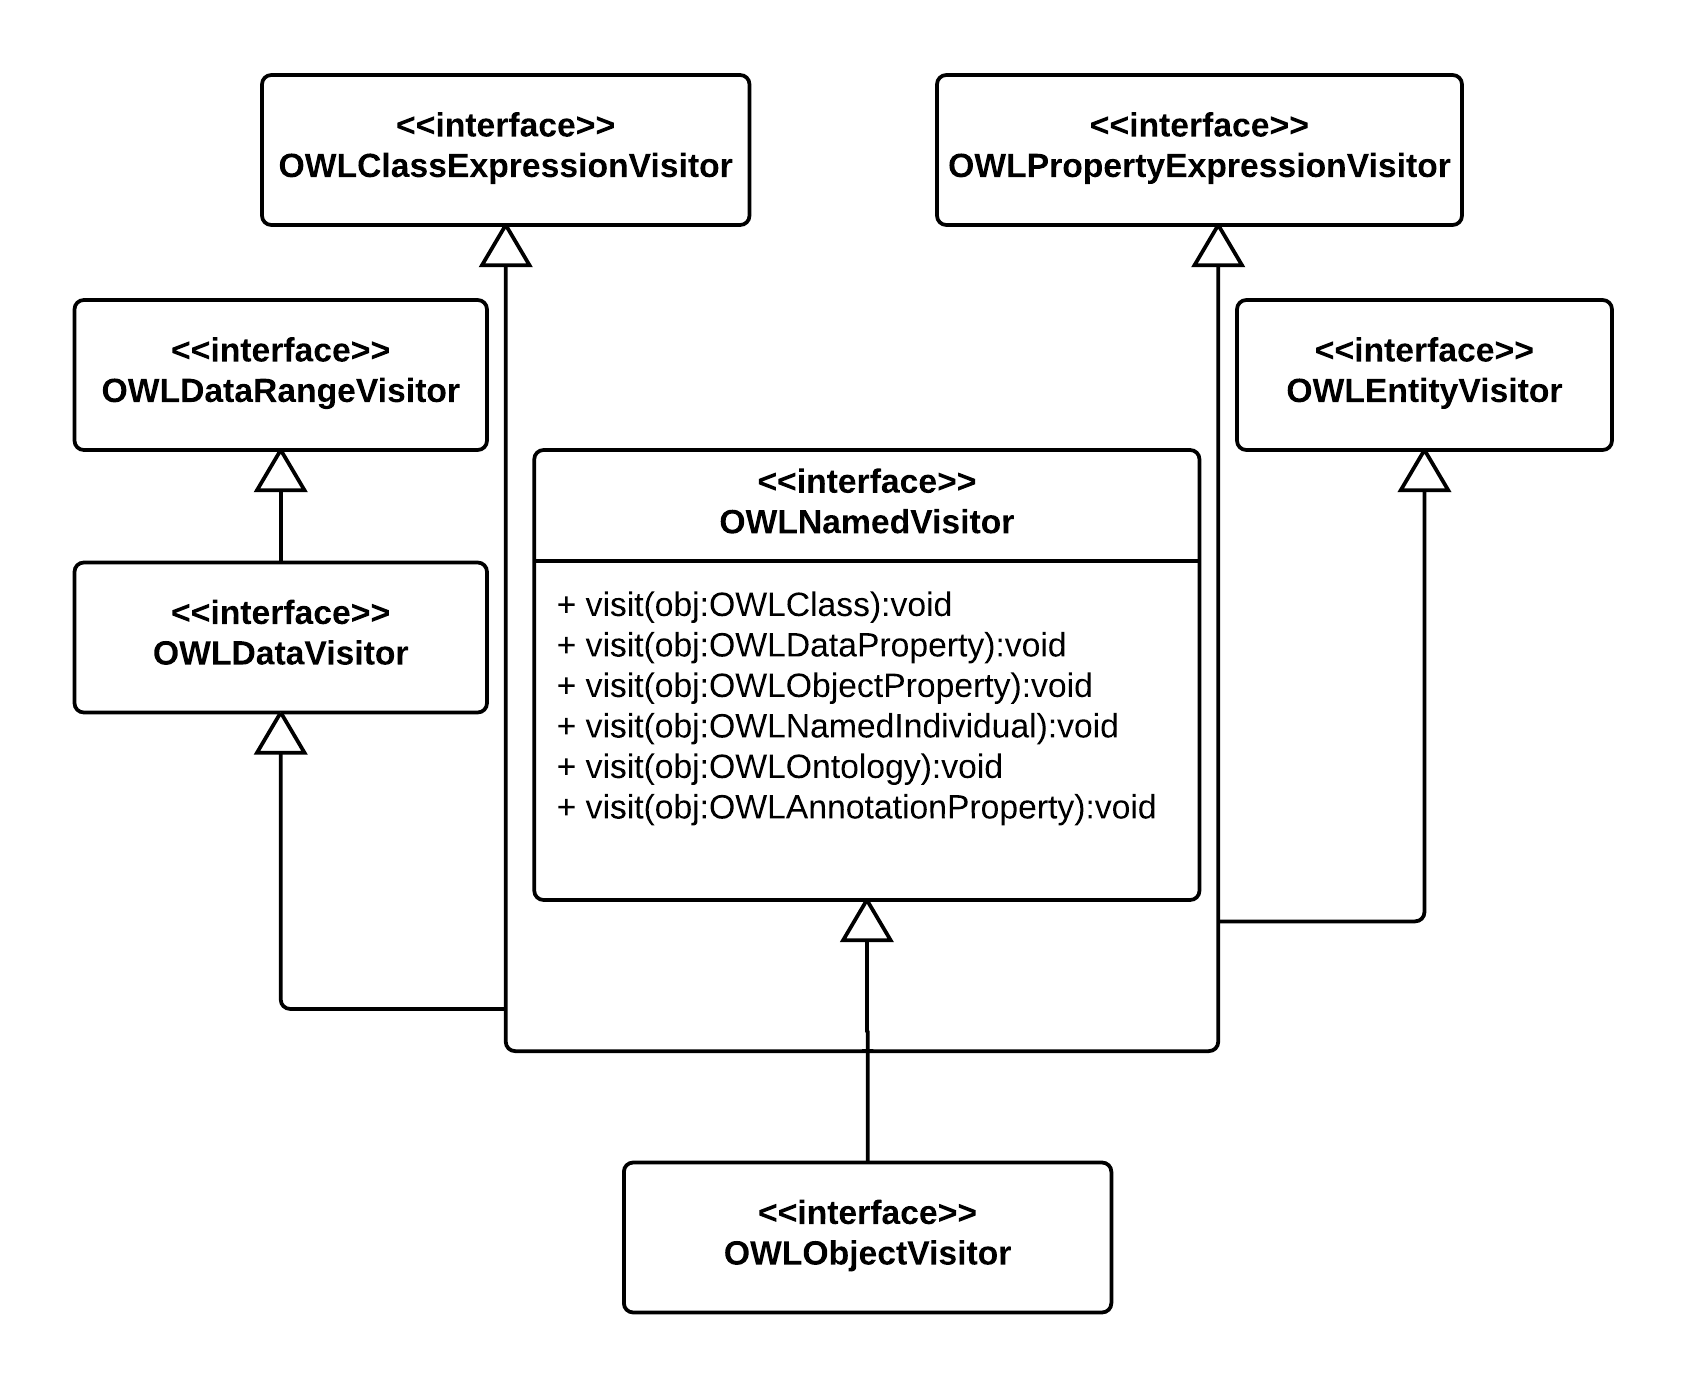
\includegraphics[width=145mm]{Figures/uml_classdiagram_owlobjectvisitor_nobackground.png}
	\caption{OWLObjectVisitor trong OWL-API \label{overflow}}
\end{figure}
Nhờ tận dụng tính đa hình trong lập trình hướng đối tượng nên các loại đối tượng thừa kế/mở rộng từ OWLObject đều có khả năng chấp nhận truy vấn lên chính nó (visitor.visit(this)) từ \textit{OWLObjectVisitor} (Hình 3.11).
\begin{figure}[h!]
	\centering
	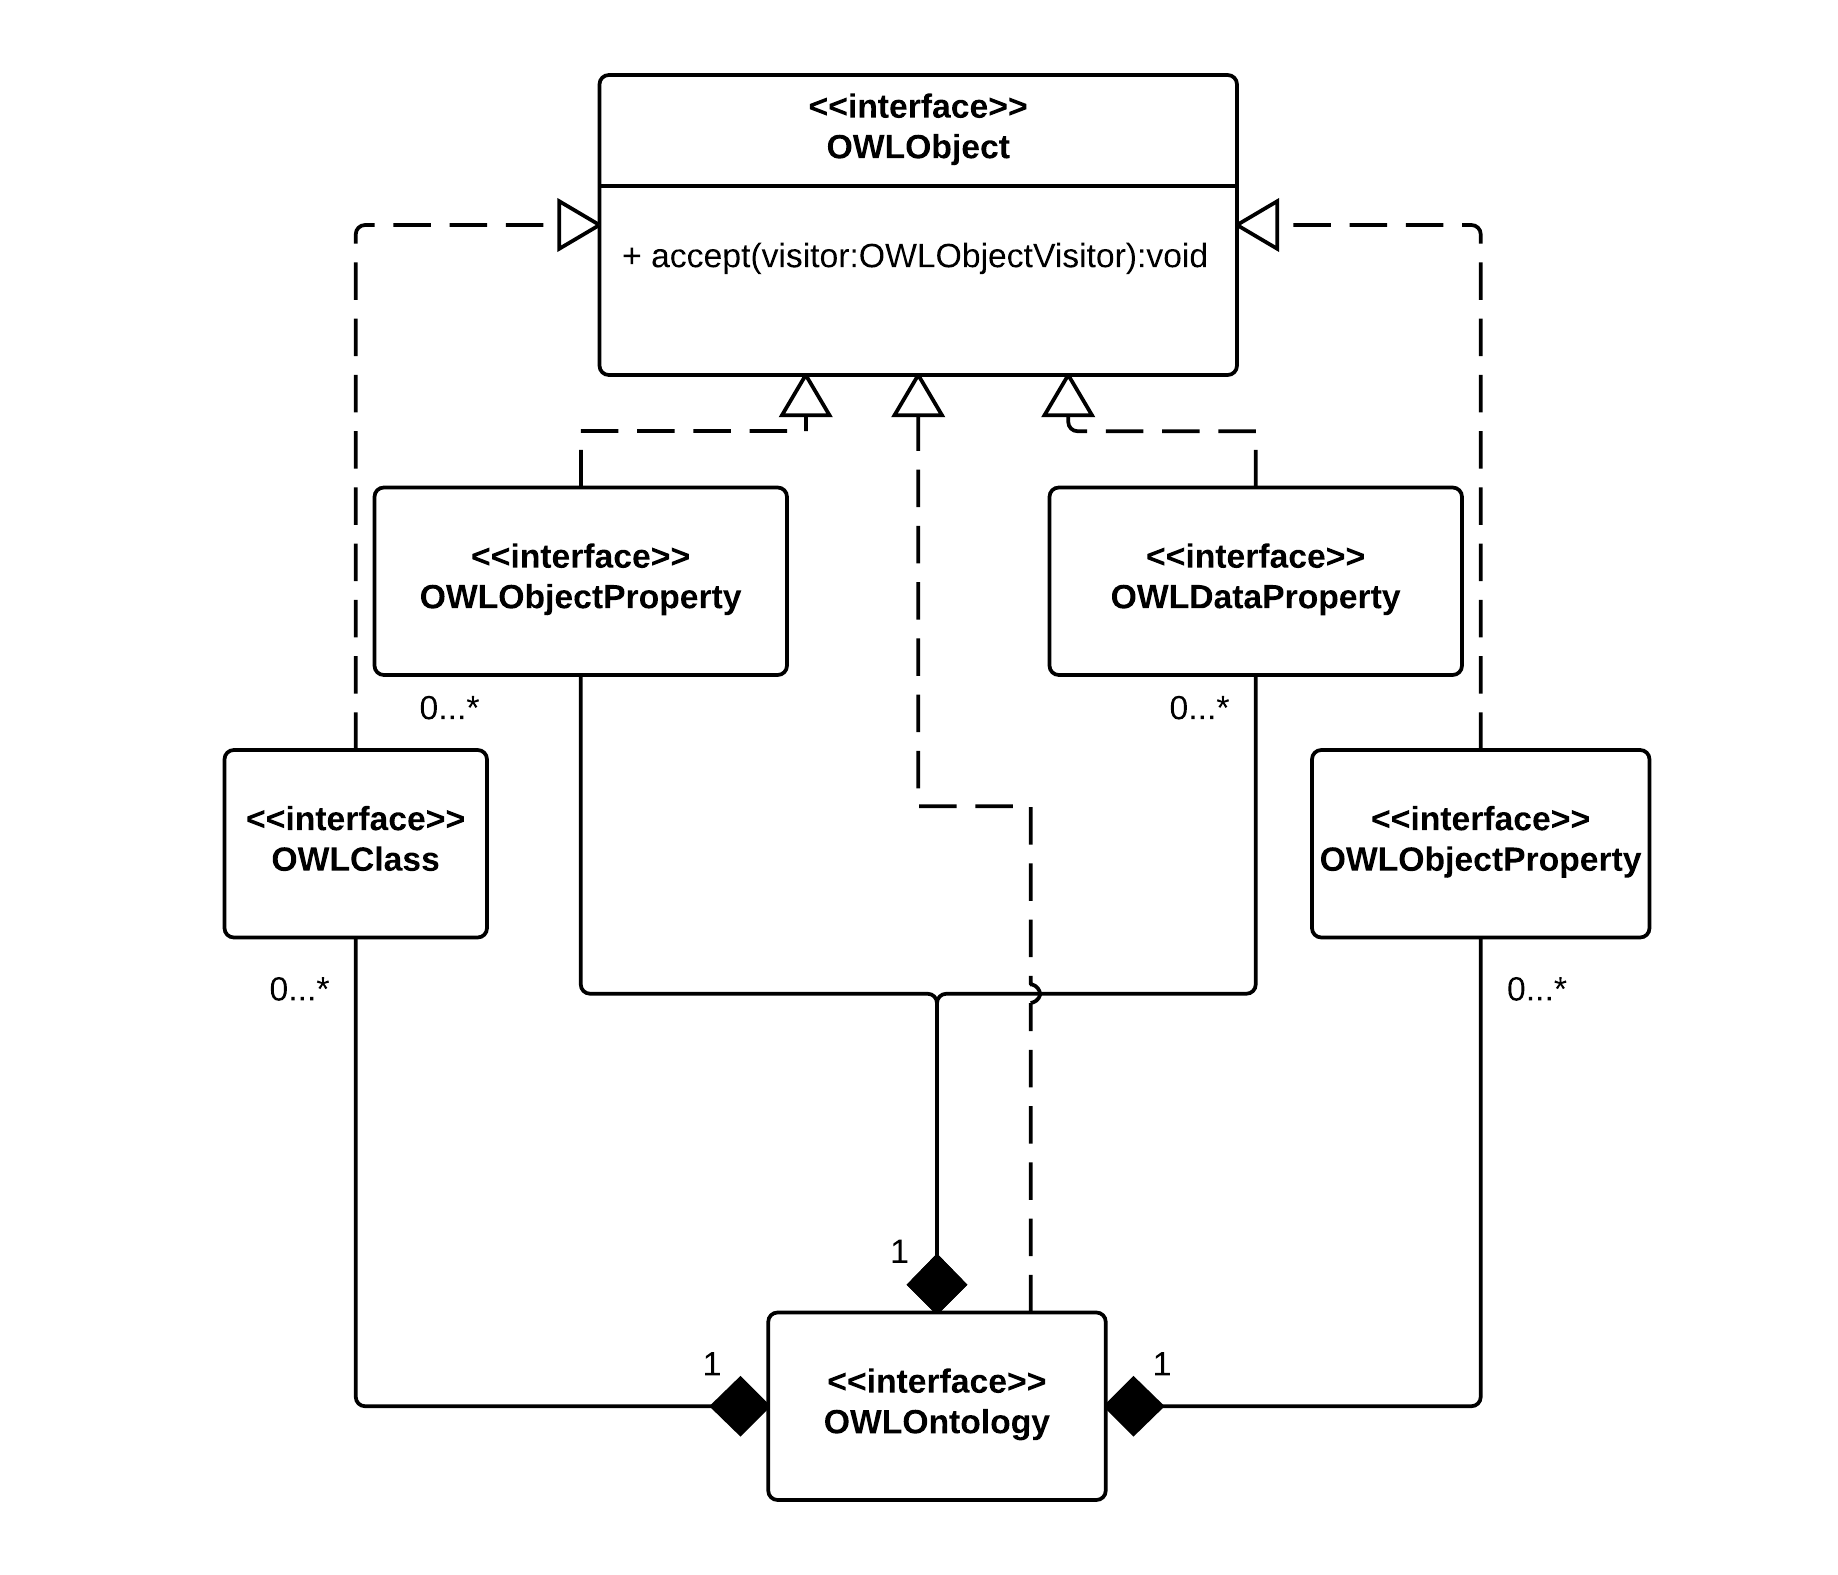
\includegraphics[width=145mm]{Figures/uml_classdiagram_owlobject_forvisitor_nobackground.png}
	\caption{OWLObject và OWLObjectVisitor trong OWL-API \label{overflow}}
\end{figure}
Để sử dụng các visitor, chúng em chỉ cần tạo các class áp dụng các interface tương ứng nhằm truy vấn dạng thành phần cụ thế như ví dụ OWLClassExpressionVisitor ở trên. Tuy nhiên, mỗi lần sử dụng là mỗi lần phải viết lại nội dung các phương thức trong Interface Visitor, để hạn chế sự lặp lại này OWL-API cũng cung cấp sẵn hoặc chúng ta cũng có thể tạo các class VisitorAdapter với nội dung mỗi phương thức được cài đặt tính năng mặc định. Ví dụ:
\begin{verbatim}
ClassExpressionVisitorAdapter implements OWLClassExpressionVistor {
  private void doNothing(OWLClassExpression ce) {};
  public void visit(OWLClass cls) {doNothing(cls);}
  public void visit(OWLObjectUnionOf union) {doNothing(cls);} ... }
\end{verbatim}
Mỗi khi muốn thay đổi nội dung phương thức nào chỉ cần \textit{Override} lại phương thức đó trong VisitorAdapter là được.
\section{Các tổ chức dữ liệu (data model) cho hệ thống}
Trong Vaadin Framework, dữ liệu trong lúc một ứng dụng đang ở trong tiến trình hoạt động được tổ chức thành các mô hình gọi là Data Model, với 3 cấp khác nhau gồm:Property, Item và Container. Có thể xem các \textit{Data Model} này như một đối tượng bao bọc (encapsulation) lại dữ liệu kiểu dữ liệu mà chúng ta muốn định nghĩa. Nếu câu hỏi là tại sao phải tốn công đưa các dữ liệu vào trong các đối tượng chứa như vậy, thì câu trả lời là vì Vaadin Framework cung cấp một cơ chế mà khi chúng ta tương tác với dữ liệu trong các \textit{Data Model} này thì đồng thời những thành phần giao diện (UI Components) cũng sẽ cập nhật các thay đổi đó. Lý do là vì hầu hết các thành phần giao diện đều được thiết kế độc lập với dữ liệu, dữ liệu được liên kết với các giao diện thông qua các \textit{Data Model} này. Sau đây chúng em xin trình bày cách tổ chức các đối tượng từ OWL-API vào trong các \textit{Data Model} là Property và Container (Item không được sử dụng vì không phù hợp với cấu trúc dữ liệu mà chúng em muốn tổ chức).

\subsection{Tổ chức các đối tượng OWL-API vào trong Property của Vaadin}
\begin{figure}[h!]
 	\centering
 	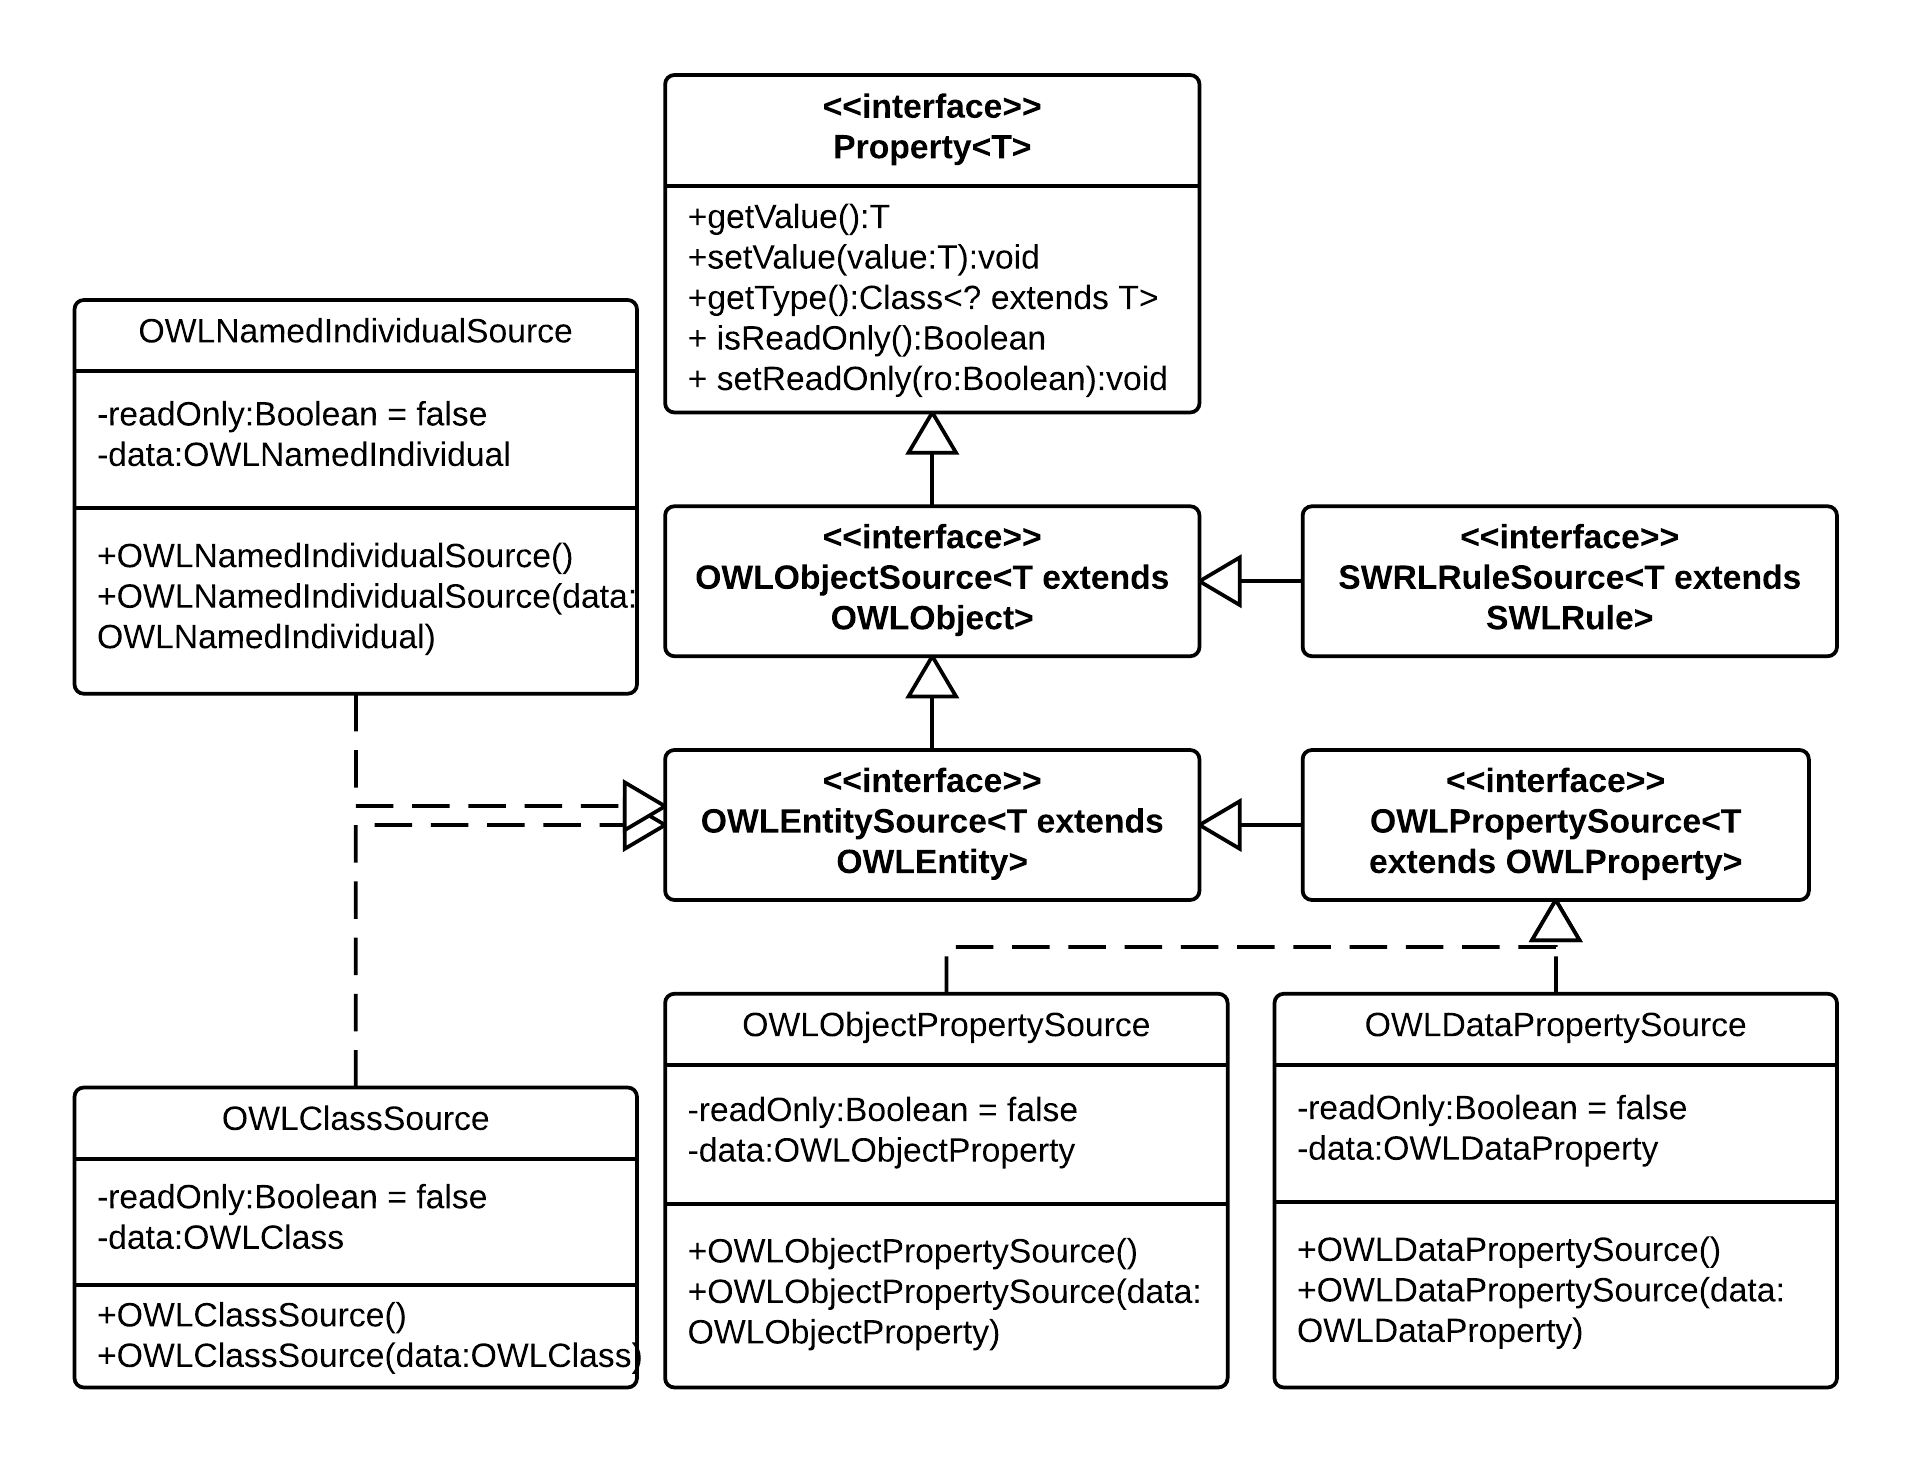
\includegraphics[width=150mm]{Figures/uml_owleditor_owlobjectsource.png}
 	\caption{Tổ chức dữ liệu dưới dạng Property \label{overflow}}
\end{figure}
\textbf{Property} là \textit{Data Model} đơn giản nhất, được Vaadin cung cấp dưới dạng Interface \textit{Property<T>} với $T$ kiểu dữ liệu được chúng ta định nghĩa, các thành phần giao diện như \textit{TextField}, \textit{Label}, \textit{TextArea} sử dụng \textit{Property} để liên kết dữ liệu với các đối tượng dữ liệu được định nghĩa qua $T$. Công việc phải làm là định nghĩa các \textit{Property} chứa các đối tượng OWL-API này. Do tính chất của OWL 2, ta có thế nói OWLClass (lớp) là một OWLEntity (thực thể), OWLEntity là một OWLObject (thành phần của OWL 2). Theo đó mà chúng em cũng sẽ tạo ra các Property tương ứng OWLObjectSource > OWLEntitySource > OWLClassSource. Việc tận dụng tính đa hình của đối tượng rất có ích khi xây dựng các UI Component chung cho các loại đối tượng giống nhau như OWLClass, OWLObjectProprerty, OWLDataProperty (cả đều mở rộng từ OWLEntity). 
\subsection{Tổ chức các thực thể OWLClass, OWLObjectProperty và OWLDataProperty thành các Container}
\begin{figure}[h!]
	\centering
	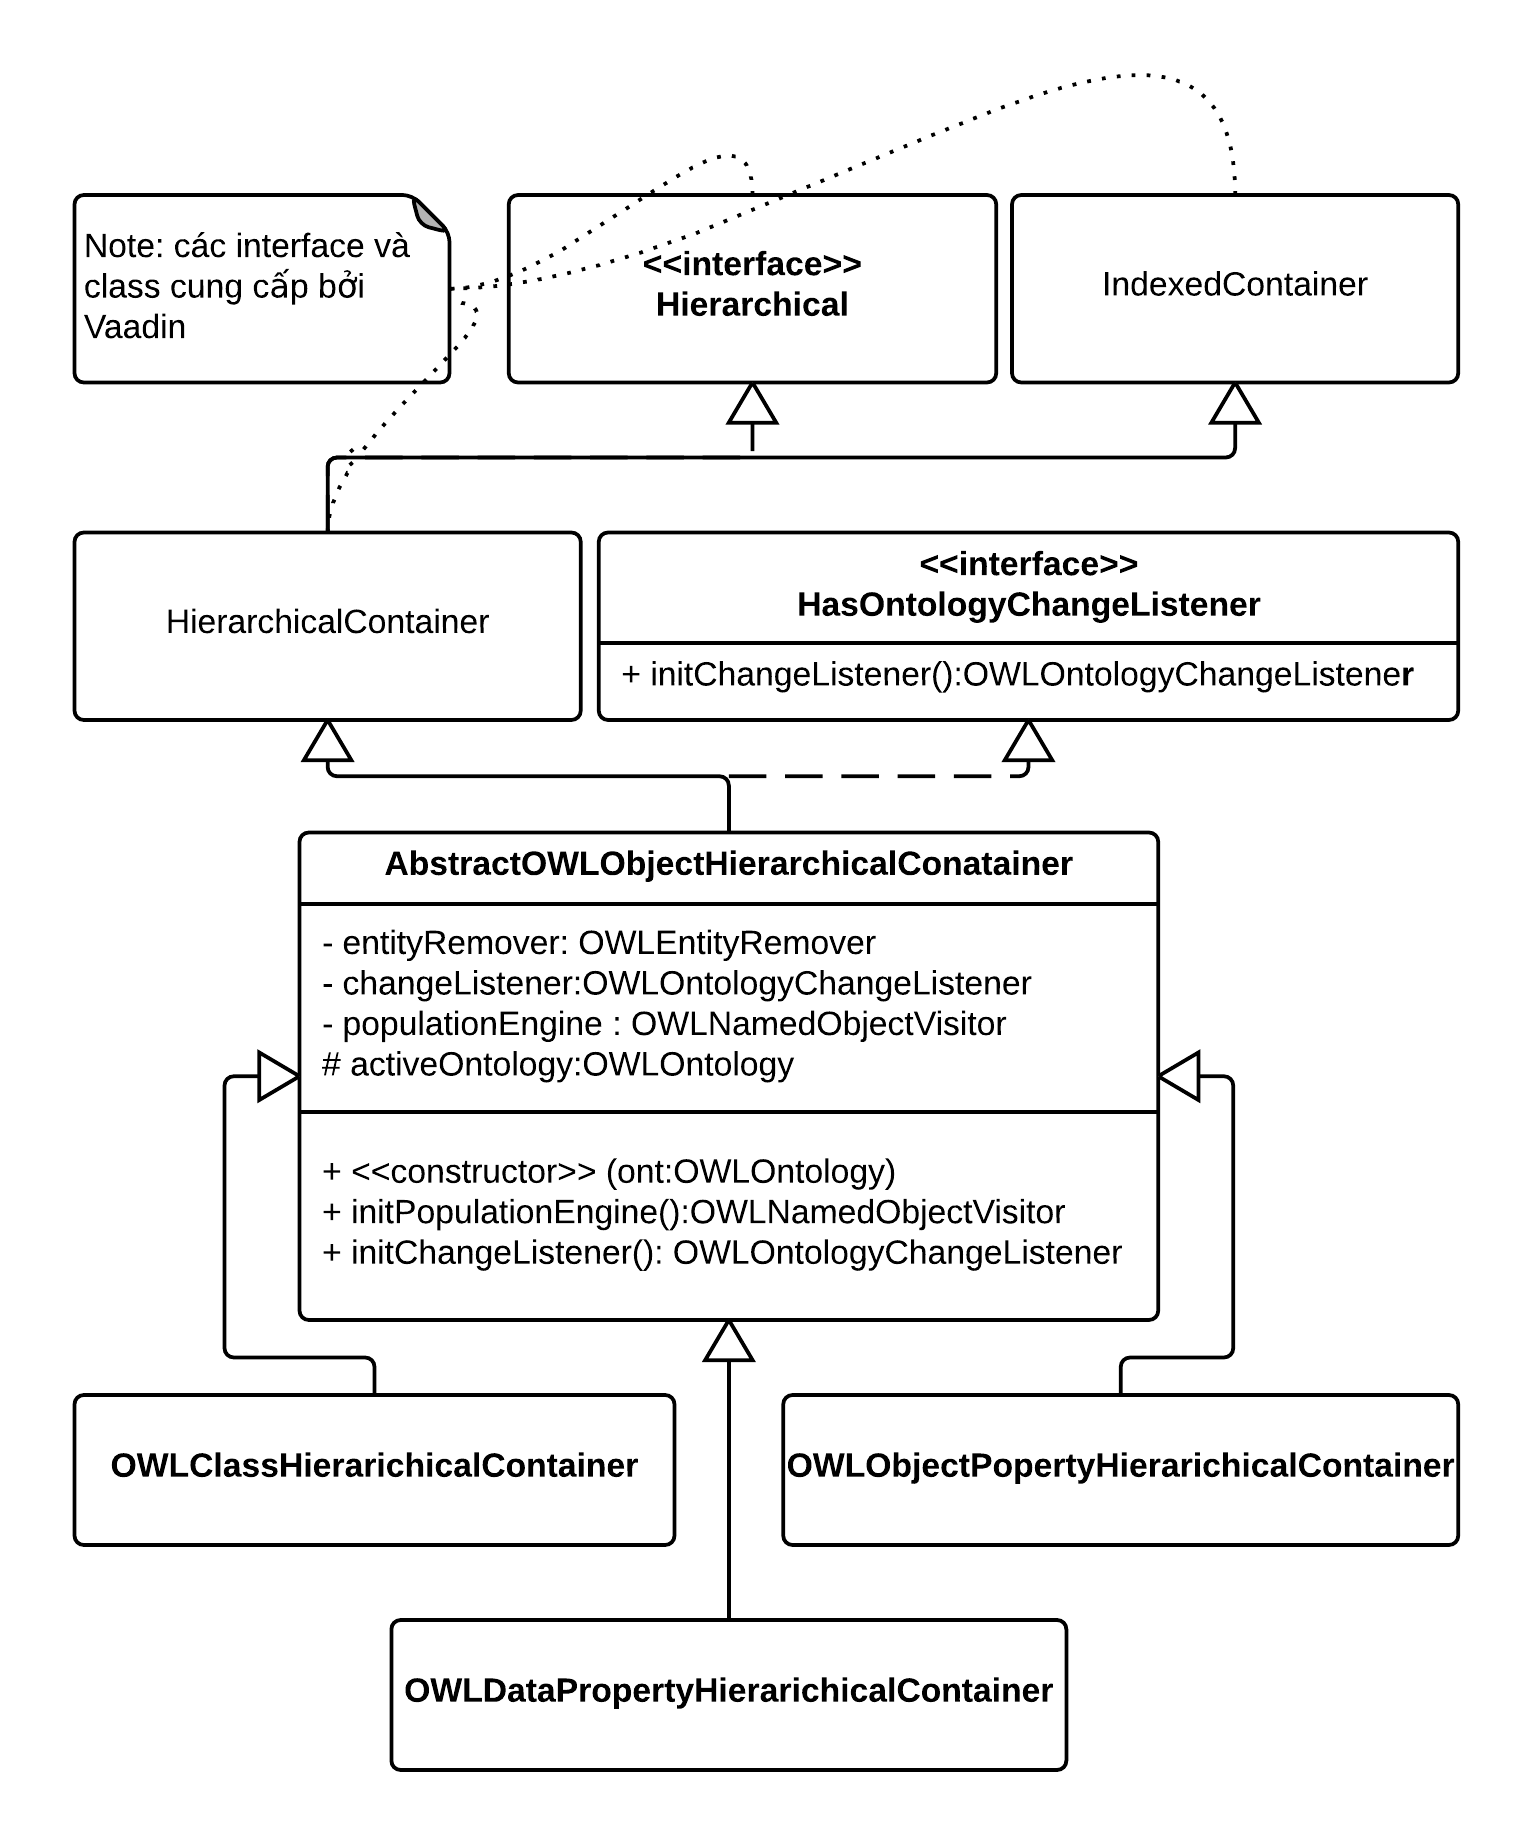
\includegraphics[width=150mm]{Figures/uml_owleditor_abstractcontainer_nobackground.png}
	\caption{Tổ chức các lớp, thuộc tính thành HierarchicalContainer \label{overflow}}
\end{figure}
\textbf{Container} là cấu trúc \textit{Data Model} phức tạp và cao nhất, chúng được chia thành các loại khác nhau tương ứng với tính chất của cấu trúc dữ liệu như \textit{HierarchicalContainer} dùng cho các cấu trúc dữ liệu phân cấp được hỗ trợ trong các thành phần giao diện (UI Component) như \textit{Table}, \textit{Tree}, \textit{ComboBox} và \textit{ListSelect}, đơn giản hơn có \textit{IndexedContainer} dùng cho cấu trúc dữ liệu dạng danh sách được hỗ trợ bởi \textit{ComboBox} và \textit{ListSelect} và \textit{JPAContainer} dùng cho các dữ liệu dạng SQL Table - hỗ trợ bở \textit{Table}, \textit{TreeTable}. Trong ứng dụng, chúng em chỉ sử dụng \textit{HierarchicalContainer} để tổ chức các lớp, thuộc tính đối tượng hay dữ liệu vì chúng cũng có tính chất phân cấp (SubClassOf, SubPropertyOf). Ở đây chúng em cũng xây dựng một AbstractClass rồi mở rộng ra với từng loại OWLEntity tương ứng là OWLClass, OWLObjectProperty và OWLDataProperty (Hình 3.13).
\section{Thiết kế cách xử lý sự kiện}
